%!TEX program = xelatex
\documentclass[12pt, b5paper]{article}
\usepackage{ctex}

\usepackage{geometry}
\geometry{b5paper,left=2cm,right=1cm,top=2.5cm,bottom=2.5cm}
\usepackage{chemformula} %化学公式宏包
\usepackage[version=4]{mhchem} %化学公式宏包
\usepackage{siunitx} %数字，单位宏包
\sisetup{
	separate-uncertainty = true,
	inter-unit-product = \ensuremath{{}\cdot{}}
} %单位间加小圆点
\usepackage{tikz} %Tikz绘图包
\usetikzlibrary{cd}
\usetikzlibrary{chains}
\usetikzlibrary{arrows}
\usetikzlibrary{arrows.meta} %画箭头
\usetikzlibrary{commutative-diagrams} %交换图
\usetikzlibrary{positioning,automata}
\usepackage[all]{xy}
\usepackage{booktabs} %三线表
\usepackage{multirow} %合并单元格
\usepackage{makecell} %表格内强制换行
\usepackage{array}
\usepackage{booktabs} %控制表格行高
\usepackage{colortbl}  %彩色表格需要加载的宏包
\usepackage{amsmath}
\usepackage{unicode-math}
\usepackage{fontspec} %字体
\newcommand*{\cred}{\textcolor{red}}

\setmainfont{Times New Roman}
\setmathfont{XITS Math}

\setlength{\parindent}{0pt} %无缩进
\usepackage{setspace}
\usepackage{fancyhdr} %设置页码
\usepackage{lastpage} %获取总页数
\pagestyle{fancy} %fancyhdr宏包新增的页面风格
\renewcommand\headrulewidth{0pt} %取消页眉中的装饰分割线
\fancyhf{}
\cfoot{\footnotesize 第 \thepage\ 页(共 \pageref{LastPage}页)}%当前页 of 总页数

\begin{document}
\begin{spacing}{1.625}

\centerline{{\huge 河北农业大学课程考试试卷}}

\centerline{\large 2022-2023学年第\underline{\ 1\ }学期}

考试科目：\underline{化学反应工程} \hfill 姓名：\underline{ \qquad \qquad} \hfill 学号：\underline{ \qquad \qquad \qquad \qquad}

学院：\underline{理工学院} \hfill 专业班级：\underline{\qquad \qquad \qquad \qquad} \hfill 卷别：\cred{A} \hfill 考核方式：\cred{开卷}

\bigskip


1. 简答题(15分)

本门课程的学习中，你对哪一章节印象最深？在这一章中学到了什么？

\bigskip
\bigskip

2. 简答题(15分)

本门课程的学习中，你觉得哪一章节学习有困难？遇到了什么困难？你认为老师在对应的教学中可以做哪些改进？

\bigskip
\bigskip

3. 简答题(16分)

浅谈你对各种类型反应器的了解。

\bigskip
\bigskip

4. 读图题(24分)

\begin{figure}[htpb]
	\centering
	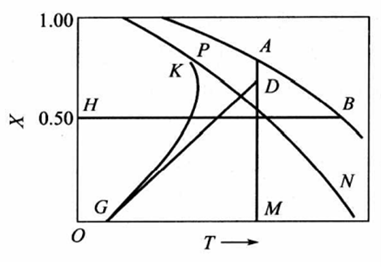
\includegraphics[width=.5\linewidth]{figures/fig1.png}
\end{figure}
上图为某反应的$T-X$关系图，其中AB为平衡曲线，NP为最佳温度曲线。

回答以下问题：

(1) 该反应为何种类型反应？

(2) 图中反应速率最大的点是哪一点？

(3) MA、GD、GK为三种不同条件下的操作线，请说明操作条件。

(4) 沿GK线操作，存在一温度最高点，这个点叫做（ \qquad ）？该点的温度与哪些因素有关？

\bigskip
\bigskip

5. 计算题(30分)

\begin{figure}[htpb]
	\centering
	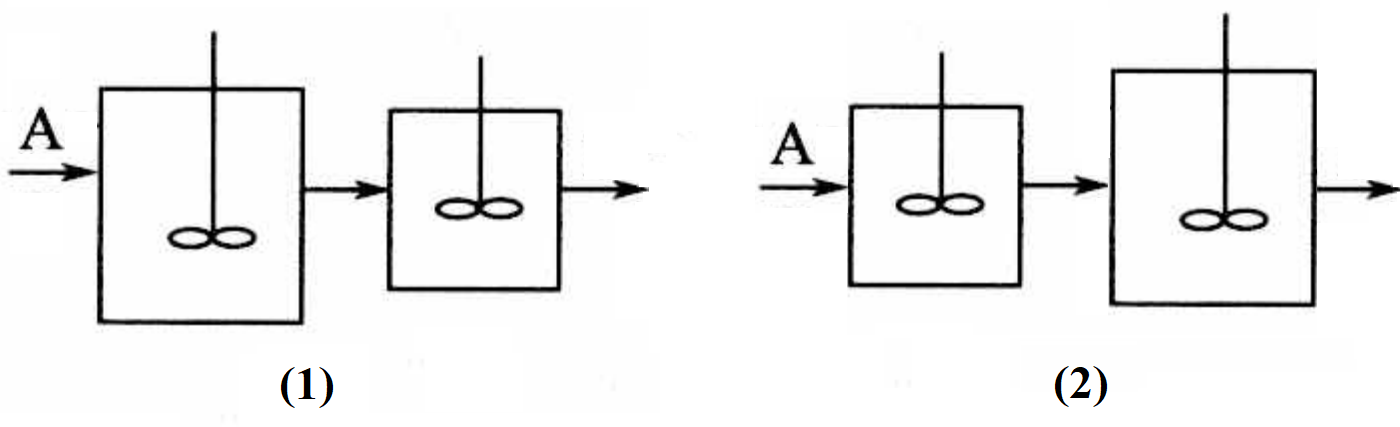
\includegraphics[width=.9\linewidth]{figures/fig2.png}
\end{figure}

如图所示，一大一小反应器以两种不同方式串联。在反应器中进行一级不可逆反应\ch{A -> R}。通过计算判断两种情况下出口最终转化率的大小。

\end{spacing}
\end{document}
